\subsubsection{DFS - Depth First Search (Busca em Profundidade)}
A busca em profundidade utiliza de recursão para visitar os nós de um grafo,
sempre indo para o nó mais profundo no grafo e quando não tiver mais nós
vizinhos para serem visitados, faz o processo de \textbf{\textit{backtracking}}
(retornar a chamada recursiva anterior)

\paragraph{Pseudo-Código: }\mbox{}\\
\begin{algorithm}[H]

	%linhas dos blocos if, for
	\SetAlgoLined
	%cria uma palavra-chave/função, primeiro arg: nome interno, segundo: nome exibido
	\SetKwFunction{DFS}{DFS} %basicamente temos o comando \DFS criado
	\SetKwProg{Fn}{Função}{:}{}
	%aqui é a estrutura de uma função sendo criada
	%\SetKwProg{comando}{texto inicial}{separador}{texto final}
	%isso é usado abaixo: \Fn que é pra definir uma função, \DFS sendo passado é a função em si, : é o que aparece na frente
	%basicamente entao eu tenho \Fn sempre define uma função, vai aparecer o nome Função: e se eu quisesse poderia colocar algo pra aparecer lá no final da função

	\Fn{\DFS{$v, adj, visitado$}}{
		$visitado[v] \gets \text{true}$\;
		\text{processar } $v$\;
		\ParaCada{$u \in adj[v]$}{
			\Se{$\neg visitado[u]$}{
				\DFS{$u, adj, visitado$}\;
			}

		}

	}
	\caption{Busca em Profundidade (DFS)}
\end{algorithm}

O funcionamento da DFS é bem intuitivo, inicialmente passamos um vértice
qualquer (geralmente os grafos são enraizados, então passamos a raíz que por
convenção é "labelada" em 0), o vetor de adjacências (isto é o grafo) e o vetor
de visitados (um vetor de booleanos que marca os vértices que já foram vistos,
isto é importante para evitar loops infinitos).

Veja a DFS funcionando de maneira mais visual, iniciando rodando $DFS(1)$:\\

\vspace{0.5cm}
\noindent % Garante que não haja recuo de parágrafo indesejado
\begin{minipage}[t]{0.31\textwidth}

	\centering

	\textbf{Passo 1: DFS(1) inicia}\\

	\vspace{0.2cm}
	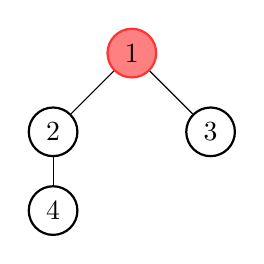
\begin{tikzpicture}[every node/.style={circle, draw, minimum size=0.5cm, thick}, visited/.style={fill=gray!30}, current/.style={fill=red!50, draw=red!80}]

		\node[current] (1) at (0, 1) {1};
		\node (2) at (-1, 0) {2};
		\node (3) at (1, 0) {3};
		\node (4) at (-1, -1) {4};
		\draw (1) -- (2);
		\draw (1) -- (3);
		\draw (2) -- (4);

	\end{tikzpicture}
	\vspace{0.2cm}
	\footnotesize
	\raggedright
	Explorando nó 1. Empilha 1. Vizinhos não visitados: 2, 3. Escolhe 2.
\end{minipage}
\hfill
\begin{minipage}[t]{0.31\textwidth}
	\centering
	\textbf{Passo 2: DFS(2) inicia}\\
	\vspace{0.2cm}
	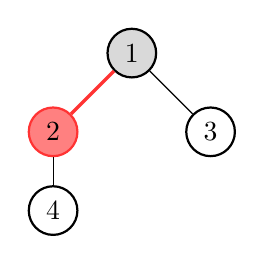
\begin{tikzpicture}[every node/.style={circle, draw, minimum size=0.5cm, thick},	visited/.style={fill=gray!30}, current/.style={fill=red!50, draw=red!80}]

		\node[visited] (1) at (0, 1) {1};
		\node[current] (2) at (-1, 0) {2};
		\node (3) at (1, 0) {3};
		\node (4) at (-1, -1) {4};
		\draw[very thick, red!80] (1) -- (2);
		\draw (1) -- (3);
		\draw (2) -- (4);
	\end{tikzpicture}
	\vspace{0.2cm}
	\footnotesize
	\raggedright
	De 1, chamou 2. Empilha 2. Vizinho não visitado: 4. Escolhe 4.
\end{minipage}
\hfill
\begin{minipage}[t]{0.31\textwidth}
	\centering
	\textbf{Passo 3: Backtrack}\\
	\vspace{0.2cm}
	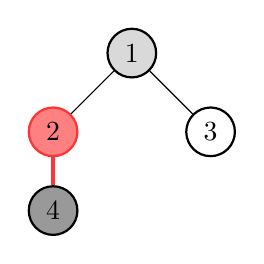
\begin{tikzpicture}[every node/.style={circle, draw, minimum size=0.5cm, thick}, visited/.style={fill=gray!30},	current/.style={fill=red!50, draw=red!80},finished/.style={fill=gray!80}]

		\node[visited] (1) at (0, 1) {1};
		\node[current] (2) at (-1, 0) {2};
		\node (3) at (1, 0) {3};
		\node[finished] (4) at (-1, -1) {4};
		\draw[visited] (1) -- (2);
		\draw (1) -- (3);
		\draw[very thick, red!80] (2) -- (4);
	\end{tikzpicture}
	\vspace{0.2cm}
	\footnotesize
	\raggedright
	De 2, chamou 4. 4 não tem vizinhos. Retorna para 2.
\end{minipage}

\noindent
\begin{minipage}[t]{0.31\textwidth}
	\centering
	\textbf{Passo 4: Backtrack}\\
	\vspace{0.2cm}
	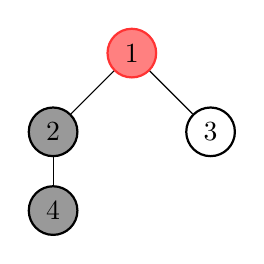
\begin{tikzpicture}[every node/.style={circle, draw, minimum size=0.5cm, thick},	visited/.style={fill=gray!30}, current/.style={fill=red!50, draw=red!80}, finished/.style={fill=gray!80}]

		\node[current] (1) at (0, 1) {1};
		\node[finished] (2) at (-1, 0) {2};
		\node (3) at (1, 0) {3};
		\node[finished] (4) at (-1, -1) {4};

		\draw (1) -- (2);
		\draw (1) -- (3);
		\draw (2) -- (4);
	\end{tikzpicture}
	\vspace{0.2cm}
	\footnotesize
	\raggedright
	Voltando pro 2 ele não tem mais vizinhos pra visitar, volta para a $DFS(1)$.

\end{minipage}
\hfill
\begin{minipage}[t]{0.31\textwidth}
	\centering
	\textbf{Passo 5: DFS(3) inicia}\\
	\vspace{0.2cm}
	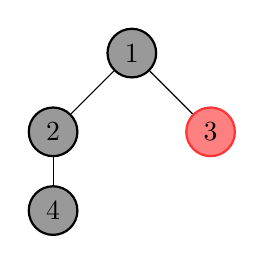
\begin{tikzpicture}[every node/.style={circle, draw, minimum size=0.5cm, thick}, visited/.style={fill=gray!30}, current/.style={fill=red!50, draw=red!80}, finished/.style={fill=gray!80}]

		\node[finished] (1) at (0, 1) {1};
		\node[finished] (2) at (-1, 0) {2};
		\node[current] (3) at (1, 0) {3};

		\node[finished] (4) at (-1, -1) {4};

		\draw (1) -- (2);

		\draw (1) -- (3);

		\draw (2) -- (4);

	\end{tikzpicture}

	\vspace{0.2cm}

	\footnotesize

	\raggedright

	Voltando pro 1 ele tem apenas o 3 para visitar, chamada $DFS(3)$ e visita o 3.

\end{minipage}
\hfill
\begin{minipage}[t]{0.31\textwidth}

	\centering

	\textbf{Passo 6: Backtrack e finalização da DFS}\\

	\vspace{0.2cm}

	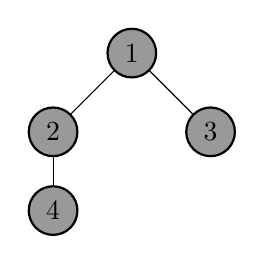
\begin{tikzpicture}[every node/.style={circle, draw, minimum size=0.5cm, thick}, visited/.style={fill=gray!30}, current/.style={fill=red!50, draw=red!80}, finished/.style={fill=gray!80}]

		\node[finished] (1) at (0, 1) {1};

		\node[finished] (2) at (-1, 0) {2};

		\node[finished] (3) at (1, 0) {3};

		\node[finished] (4) at (-1, -1) {4};

		\draw (1) -- (2);

		\draw (1) -- (3);

		\draw (2) -- (4);

	\end{tikzpicture}

	\vspace{0.2cm}

	\footnotesize

	\raggedright

	Ao visitar o 3, ele não tem mais vizinhos, logo encerrou-se tudo.

\end{minipage}

Veja que nessa ordem de visitação temos: $[1, 2, 4, 3]$.
\paragraph{Implementação: }\mbox{}
Vejamos a implementação da DFS em Python e em C++.

\textbf{Python: }
\begin{lstlisting}[language=Python, basicstyle=\ttfamily\small, frame=single, numbers=left, showstringspaces=false]
		
		def dfs(u, adj, visited):
			visited[u] = True
			print(u) # Processa o vertice atual

			for v in adj[u]:
			if not visited[v]:
				dfs(v, adj, visited)
	\end{lstlisting}
\vspace{0.3cm}
\textbf{C++:}
\begin{lstlisting}[language=C++, basicstyle=\ttfamily\small, frame=single, numbers=left, showstringspaces=false]
		
		void dfs(int u, const vector<vector<int>>& adj, vector<bool>& visited) {
			visited[u] = true;
			// Processa o vertice atual aqui
			for (int v : adj[u]) {
				if (!visited[v]) {
					dfs(v, adj, visited);
				}
			}
		}
\end{lstlisting}